\section{Systemtest med kendt input}
I dette afsnit vil det samlede system blive testet, så det er muligt at se, om systemet behandler dette input, som det forventes. På baggrund af disse målinger er det muligt at konkludere, om systemet virker. 

\subsection{Beskrivelse}
For at teste accelerometer-signalerne indsendes der to spændinger svarende til de to accelerometre. Denne varireres over tid, således at spændingen svarer til $90-180^{\circ}$. Derudover testes det for om vinkel falder til $-200^{\circ}$, når spændingen svarende til $180^{\circ}$ overskrides. 

For at teste om det samlede system med et kendt input benyttes en funktionsgenerator, så der kan genereres et sinussignal på $500~Hz$ med en peak-peak-amplitude på $4~mV$. Sinussignalets frekvens og amplitude er nær ved, hvad der kan forventes af et filtreret EMG-signal. Outputtet fra sinussignalet er filtreret gennem det implementerede lavpasfilter. 


Hele testen foretages i 10 sekunder og optages via mikrokontrolleren. Ud fra disse målinger, er det muligt at se effekten af systemets blokke, når de er sammensat ved at sammenligne input-signalet og outputtet af det samplede sinussignal samt spændingerne for det samlede acclerometre. Resultaterne fra målingerne visualiseres i MATLAB. 


\subsection{Resultater af test}
Fra testen plottes og visualiseres systemets input af det samplede sinussignal og outputtet fra det opsamlede digitalt filtrerede signal, samt spændingen fra de to accelerometre, der er omregnet til en samlet vinkel ved lineær interpolation. Derudover er der plottet det opsamlede digitale output som er behandlet i EMG-algortimen. Resultaterne fremgår af \autoref{fig:test_kendtinput_vinkel}. 

\begin{figure}[H]
\centering
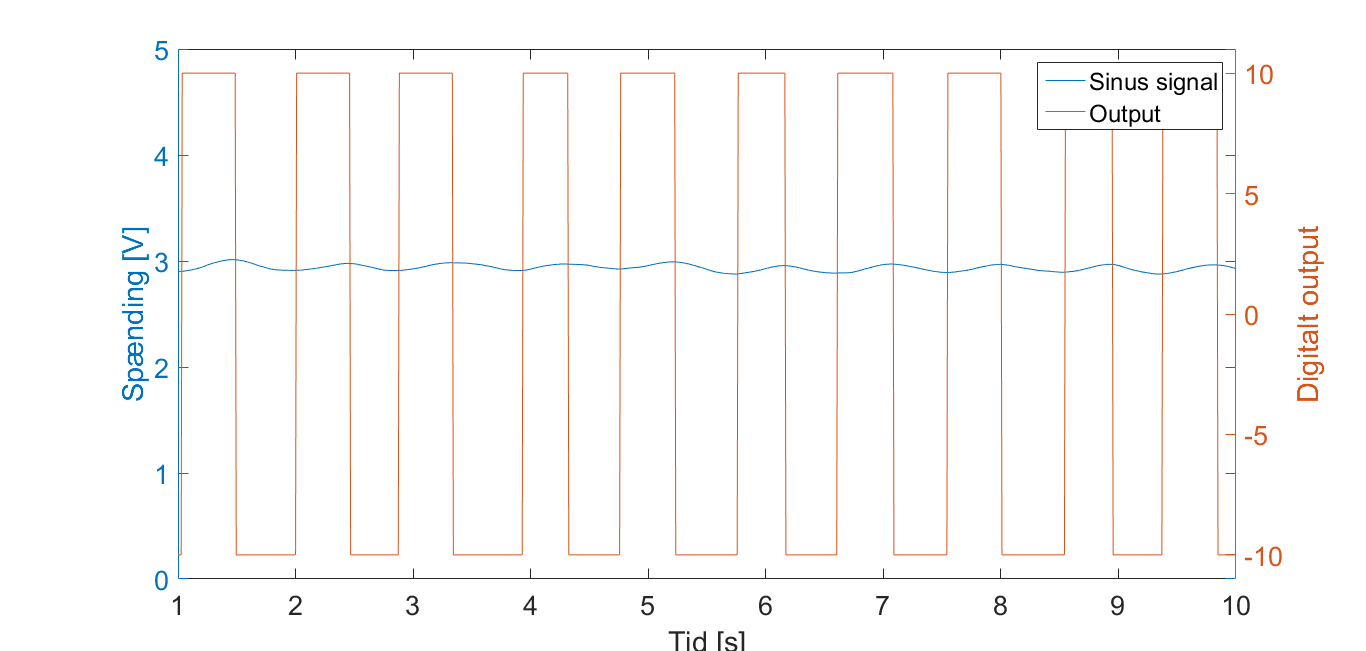
\includegraphics[width=0.4\textwidth]{figures/kontrol_test_sinus}
\caption{På den øverste figur illustrerer den blå graf den samlede vinkel. Det fremgår af grafen at vinkelen er stigende fra $90^{\circ}$ til $175^{\circ}$, hvorefter vinklen daler markant ned til $-115^{\circ}$. 
På den midterste figur, illustrer den blå graf det opsamlede inputsignal, svarende til en sinus på $500~Hz$ med en $V_{pp}$ på $4~mV$. Den røde graf illustrer det opsamlede digitale outputsignal, disse værdier er målt i spændingen. 
På den nederste figur illustrerer den blå graf signalets digitale output. Signalet går fra $10$ ved stigende muskelaktivitet til $-10$ ved en faldende muskelaktivitet, hvis grafen går i $0$ svarer dette til en overskridelse af en vinkel på $180^{\circ}$.}
\label{fig:test_kendtinput}
\end{figure}

På baggrund af målingerne for den øverste figur på \autoref{fig:test_kendtinput} fremgår det, at en stigende spænding svarende til $90-175^{\circ}$, får den samlede vinkel til at stige. Ved en vinkel på $175^{\circ}$ overskrider denne spændingen svarende til en vinkel på $180^{\circ}$, hvor vinklen daler markant på $1~ms$ ned til $-115^{\circ}$. 
Dette burde ifølge det implementerede kode gå ned til en vinkel på $-200^{\circ}$ ved overskridelse af $180^{\circ}$.
Disse faktorer er angiveligt fordi den målte spænding ikke har været $0~V$ ved forsøgets begyndelse, hvorfor den samlede vinkel ikke når den maksimale vinkel på $180^{\circ}$ og ikke daler til $-200^{\circ}$.

Det fremgår af den midterste figur og den nederste figur på \autoref{fig:test_kendtinput}, at der er en sammenhæng mellem det opsamlede filtrerede sinussignal og det opsamlede outputsignal. Når sinussignalet er faldende, daler outputsignalet markant fra $10$ til $-10$, hvorefter outputsignalet stiger markant fra $-10$ til $10$, når signussignalet stiger igen. Derudover ses det, at tiden hvor signalet befinder sig i $10$ eller $-10$ varierer alt efter hvor længe det opsamlede filtrerede sinussignals er stigende eller faldende .

På den nederste figur på \autoref{fig:test_kendtinput} fremgår det at efter have befundet sig i $-10$ ved 9 sekunder, stiger til $0$. Dette er grundet målingerne i den øverste figur, hvor vinkelen når $175^{\circ}$. Dette stemmer overens med at, hvis vinklen  overskrider de $180^{\circ}$ skal det opsamlede digitale signal gå i $0$. 